
\subsubsection{Problem definition}

If there are 2 materials with different thermal expansions the volume changes of the materials will be uncommon. The material with the higher thermal expansion expands more than the material with the low thermal expansion. If deformations at the outer boundaries are prevented, different states of stress will occur in these two materials. But the stresses perpendicular to the parting plane must be equal. The values of the stresses as a result of temperature changes can also easily be calculated by the HOOKE's linear elastic model. The aim of this simulation is to specify the stresses at several areas in the solid. Fig. \ref{fig64} shows a sketch of the calculation area.

\begin{figure}[htbp]
\centering
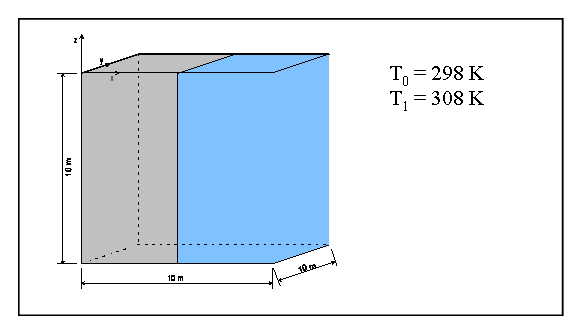
\includegraphics[width=0.6\textwidth]{TM/figures/fig64.eps}
\caption{Calculation area with two different materials}
\label{fig64}
\end{figure}

%\newpage

\subsubsection{Model set-up of the 3~D numerical model}

The calculation was done with a 3~D model. The $xy$-plane is the horizontal plane. The height of the body is in $z$-direction. The dimensions of this 3~D model are 10~m in all directions. The model includes 1000 elements and 1331 nodes. Deformations perpendicular to the outer surfaces are suppressed. Deformations in $x$- and $z$-direction are suppressed. The initial temperature in the whole area is 298~K. At the top and at the bottom of the model thermal boundary conditions are set with a temperature of 308~K. Thereby the heating of the body about 10~K is simulated. The used parameters of the solids represent the material behaviour of concrete. The calculation is divided in 1000 time steps with a constant time step length of 0.5 seconds. A sketch of the calculation model is shown in Fig. \ref{fig65}.

\begin{figure}[htbp]
\centering
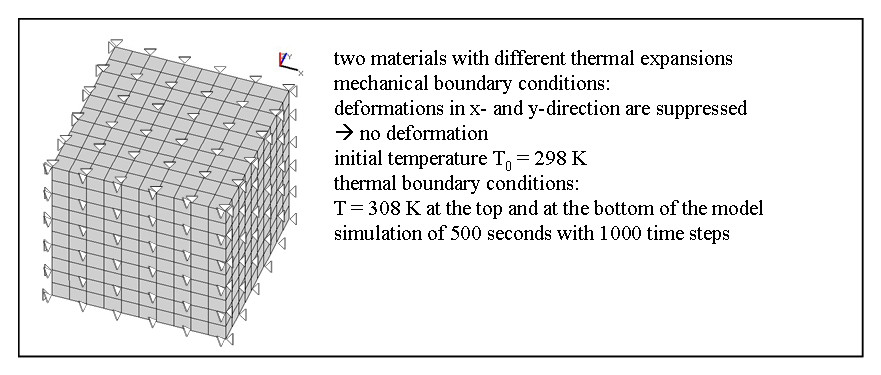
\includegraphics[width=0.9\textwidth]{TM/figures/fig65.eps}
\caption{Calculation model (3D) with 2 materials}
\label{fig65}
\end{figure}

\begin{table}[htbp]
\centering
\begin{tabular}{|c|l|l|}
\hline
symbol & quantity & value \\
\hline
$T_0$  & Initial temperature (before heating) & 298 K \\
\hline
$T_1$  & Temperature after heating & 308 K \\
\hline
$\rho$  & Density of the solid &  2.2 t$\cdot$m$^{-3}$  \\			
\hline
$E$ & Young's modulus of the solid & 25 GPa \\
\hline
$\nu$ & Poisson ratio & 0.27 \\
\hline
$\alpha_1$ & Thermal expansion of material 1 & 6.0$\cdot$10$^{-6}$ K$^{-1}$ \\
\hline
$\alpha_2$ & Thermal expansion of material 2 & 1.2$\cdot$10$^{-5}$ K$^{-1}$ \\
\hline
$c$      & Thermal capacity & 1.0 J$\cdot$kg$^{-1}\cdot$K$^{-1}$ \\
\hline
$\kappa$ & Thermal conductivity & 1.0 W$\cdot$m$^{-1}\cdot$K$^{-1}$ \\
\hline
\end{tabular}
\caption{Used parameters}
\label{tab62}
\end{table}

%\newpage

\subsubsection{Evaluation method}

The equations of the mechanical behaviour base on the HOOKE's law for linear elastic materials (see Eqns. \ref{eq61} to \ref{eq63}). The analytical solution can be derived from these time independent equations with the assumptions of suppressed deformations in $y$- and $z$-direction and an isotropic thermal expansion:
\begin{displaymath}
\varepsilon_x\,=\,\varepsilon_z\,\equiv\,0
\end{displaymath}
Additionally the stresses in x-direction (perpendicular to the parting plane between the two materials) must be equal:
\begin{displaymath}
\sigma_{x1}\,=\,\sigma_{x2}
\end{displaymath}
Further the expansion of the one material leads to a compression of the other material with the same value in x-direction:
\begin{displaymath}
\varepsilon_{x1}\,=\,-\varepsilon_{x2}
\end{displaymath}
With these limiting conditions the analytical solutions are:
\begin{eqnarray}
\varepsilon_{x1} & = &
\frac{\Delta T}{2}\cdot\left(\alpha_1-\alpha_2\right)\cdot
\left(\frac{1+\nu}{1-\nu}\right)
\label{eq65} \\[1.5ex]
\varepsilon_{x2} & = & -\varepsilon_{x1}\,=\,
-\frac{\Delta T}{2}\cdot\left(\alpha_1-\alpha_2\right)\cdot
\left(\frac{1+\nu}{1-\nu}\right)
\label{eq66} \\[1.5ex]
\sigma_{x1} & = & \sigma_{x2}\,=\, E\cdot
\frac{\varepsilon_{x2}\cdot\left(1-\nu\right)-\alpha_2\cdot\Delta T\cdot\left(1+\nu\right)}{1-\nu-2\nu^2}
\label{eq67} \\[1.5ex]
\sigma_{y1} & = & \sigma_{z1}\,=\,
\frac{\nu\cdot\sigma_{x1}-\alpha_1\cdot\Delta T\cdot E}{1-\nu}
\label{eq68} \\[1.5ex]
\sigma_{y2} & = & \sigma_{z2}\,=\,
\frac{\nu\cdot\sigma_{x2}-\alpha_2\cdot\Delta T\cdot E}{1-\nu}
\label{eq69}
\end{eqnarray}
{\small
indices:

\begin{tabbing}
\=xxxx  \=xxxxxxxxxxxxxxxxxxxxxxx \kill
\> 1 -- \> material 1 \\[1.0ex]
\> 2 -- \> material 2
\end{tabbing}
}

Eqns. \ref{eq65} to \ref{eq69} provide the strains and stresses after heating the body of two materials. The state of stress is anisotropic.

\subsubsection{Results}

With the analytical solution in Eqns. \ref{eq65} to \ref{eq69} and the used parameters the values of the strains in $x$-direction at the parting plane amount
\begin{eqnarray*}
\varepsilon_{x1} & = & -5.219178\cdot 10^{-5} \\[1.5ex]
\varepsilon_{x2} & = & \phantom{-}5.219178\cdot 10^{-5}
\end{eqnarray*}
The values of the stresses are
\begin{eqnarray*}
\sigma_{x1} & = & \sigma_{x2}\,=\,-4891304.34\,\mathrm{Pa}
                             \,=\,-4.8913\,\mathrm{MPa} \\[1.5ex]
\sigma_{y1} & = & \sigma_{z1}\,=\,-3863907.08\,\mathrm{Pa}
                             \,=\,-3.8639\,\mathrm{MPa} \\[1.5ex]
\sigma_{y2} & = & \sigma_{z2}\,=\,-5918701.60\,\mathrm{Pa}
                             \,=\,-5.9187\,\mathrm{MPa}
\end{eqnarray*}
This anisotropic state of stress is reached after the whole body is heated. The temporal stress developments in several nodes calculated with both RockFlow and \linebreak
GeoSys/RockFlow are presented in Fig. \ref{fig66} and Fig. \ref{fig67}.

\begin{figure}[htbp]
\centering
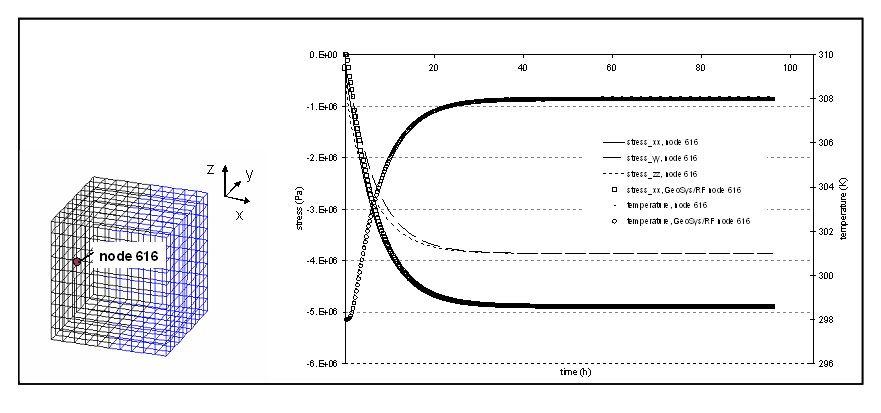
\includegraphics[width=0.9\textwidth]{TM/figures/fig66.eps}
\caption{Temporal stress development in node 616}
\label{fig66}
\end{figure}

\begin{figure}[htbp]
\centering
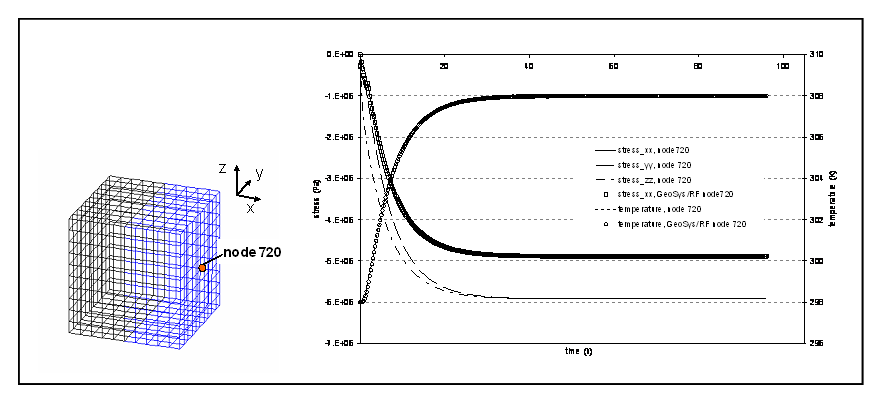
\includegraphics[width=0.9\textwidth]{TM/figures/fig67.eps}
\caption{Temporal stress development in node 720}
\label{fig67}
\end{figure}

The results of the 3 D simulation show an exact agreement with the analytical solutions.

\begin{tabular}{|l|l|l|l|}
\hline
Path in the & Used code	& Used version & Date of simu- \\
benchmark deposit	& & & lation run \\
\hline	
TM$\backslash$heating$\backslash$cube$\backslash$	& GeoSys/RockFlow	& RockFlow 4, & Dec. 2007 \\
2\_mat$\backslash$GeoSys/RockFlow$\backslash$	& & rf4-507 & \\
tm\_02\_3Du	& & & \\
\hline	
\end{tabular}
